\chapter{Methodology and Implementation}
\label{chap:implementation}
 
In this chapter the implementation developed for the GraphSLAM algorithm is presented and explained. The implementation is capable of solving the SLAM problem in an offline manner for a 2D scenario, in the cases of known and unknown data association.

The g$^2$o framework used in this work provides of a least squares solver for the optimization of equation~\eqref{eq:minimization}, as well as a protocol to define a graph in the SLAM problem. g$^2$o is well optimized and it has several options for the solver, so the known correspondence version of the GraphSLAM algorithm is relative straightforward to implement.

However, g$^2$o doesn't provide a way to handle unknown data association, so the main goal of this work is to implement a method for solving the correspondence problem in an efficient manner.

\section{The g$^2$o Protocol}

The first step to implementing the GraphSLAM algorithm is to define a protocol to store and interpret the data on a graph. g$^2$o already provides such protocol. The stored data are of two types: data from nodes, and data from edges. 

In the SLAM context, nodes itself can be of two types, pose nodes and landmark nodes. Pose nodes represent the pose of the robot, in the 2D case they consist in 3 variables: robot's $x$ and $y$ position, and robot's orientation $\theta$. In g$^2$o a pose node is denoted with the keyword \texttt{VERTEX\_SE2}\footnote{Vertex is synonymous of node. SE2 is the Non-Euclidean space that consists of two spatial dimensions and a angular dimension.}. Landmark nodes represent the 2D position ($x$ and $y$) of a landmark. They are denoted with the keyword \texttt{VERTEX\_XY}.

Edges represents either robot's odometry (data of robot's change in position), or robot's measurements of landmarks. Odometry is measured as the difference between robot's pose at two consecutive timesteps: $(\Delta x, \Delta y, \Delta \theta)$. On the other hand, robot measurement are given as the $x$ and $y$ distance to the landmark relative to the robot reference frame. Figure~\ref{fig:protocol} illustrates the odometry an measurement of a robot. Keywords \texttt{EDGE\_SE2} and \texttt{EDGE\_SE2\_XY} are use to denote odometry and measurement edges respectively.

\begin{figure}[htbp!]
    \centering
    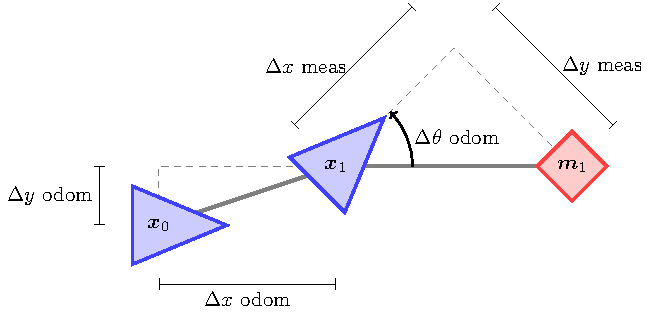
\includegraphics[width=0.7\textwidth]{tikz/protocol.pdf}
    \caption{Ilustration of odometry and measurements values in g$^2$o.}
    \label{fig:protocol}
\end{figure}

For GraphSLAM to work correctly, one must also provide to the algorithm of the uncertainty of odometry and measurements. These correspond to the covariance matrices $\bs{R}_k$ and $\bs{Q}_k$ from motion~\eqref{eq:motion-model} and measurement~\eqref{eq:measurement-model} model respectively. g$^2$o works with the inverse of the covariance matrix, known as the information matrix however, but these representation are equivalent in terms of the knowledge of the system. Since covariance matrices (and their inverse) are symmetric, only the upper diagonal elements are needed. In this work it is assumed that the model's uncertainly are time independent, i.e., all nodes have the same values for the information matrix. The notation of each element of the matrices is given by:

\begin{equation}
    \bs{R}^{-1}_k = \begin{pmatrix}
    ipxx & ipxy & ipxt\\
    ipxy & ipyy & ipyt\\
    ipxt & ipyt & iptt
    \end{pmatrix} \;\;
    \bs{Q}^{-1}_k = \begin{pmatrix}
    ilxx & ilxy\\
    ilxy & ilyy
    \end{pmatrix} 
    \label{eq:info-matrices}
\end{equation}

Finally, nodes must be indexed so they can be distinguishable form one another. This is indicated by an integer \texttt{id}. Ids are used in edges to indicate which two nodes the edge is connecting.

Table~\ref{tab:protocol} summarize the g$^2$o notation to represent nodes and edges.

\begin{table}[htbp!]
    \centering
    \begin{tabular}{|c|c|}
        \hline
        Graph element & Notation\\
        \hline
        Pose node & \texttt{VERTEX\_SE2 id x y t}\\
        Landmark node & \texttt{VERTEX\_SE2\_XY id x y}\\
        Odometry edge & \texttt{EDGE\_SE2 id1 id2 dx dy dt ipxx ipxy ipxt ipyy ipyt ipyy}\\
        Measurement edge & \texttt{EDGE\_SE2\_XY id1 id2 dx dy ilxx ilxy ilyy}\\
        \hline
    \end{tabular}
    \caption{g$^2$o protocol for node and edge definition.}
    \label{tab:protocol}
\end{table}

In this work, it is assumed that the first pose is known with absolute certainty, and is fixed to $(0,0,0)$. In g$^2$o, this is done by the command \texttt{FIX id}, where the id of the first pose is used. Aside of the first pose, it is assume that only information about robot odometry and measurement is provided, so only data from edges is known. 

To use the data in the framework, it can be written in a plain text, which is then uploaded to g$^2$o.

\section{The Known Correspondence Case}

In the known correspondence case each measurement incorporates the information of the landmark sensed form the map. It's equivalent to know the correct values of \texttt{id1} and \texttt{id2} for every \texttt{EDGE\_SE2\_XY}. In a real world scenario, data association is usually not known, however, the known correspondence case is still useful in simulations to check the correctness of the algorithm.

With g$^2$o, solving the known correspondence case is just a matter of loading the data to the framework, set the desired parameters, and running the solver. 

The parameters that can be set in the solver includes: 

\begin{enumerate}
    \item The sparse solver for the inversion in~\eqref{eq:linear-system}: Cholesky solver, PCG solver
    \item The optimization algorithm for solving~\eqref{eq:linearized}-\eqref{eq:update}: Gauss-Newton, Levenberg-Marquardt
    \item The number of iteration for the algorithm to stop.
\end{enumerate}

For the sparse solver, g$^2$o uses third-parties libraries from which the user can choose: CHOLMOD, CSparse\footnote{CHOLMOD and CSparse can be found in \url{http://faculty.cse.tamu.edu/davis/suitesparse.html}}, Eigen\footnote{\url{http://eigen.tuxfamily.org/index.php?title=Main_Page}}. 

This work provides of a Python script to easily set the parameters of the framework and run the solver. It also provides of a 2D simulator that generates a robot path, landmarks and measurements. It's a modified version of the g$^2$o simulator that allows the user to set the information parameters from matrices~\eqref{eq:info-matrices} in the simulations. This make possible to test the GraphSLAM algorithm for different noise levels. The simulation also allows to compare the results with the ground truth. The ground true estimate to be achieved, and it's given by the simulator. 

The Python script is also able to generate an initial guess of the estimate using robot odometry and the first measurement of each landmark. The initial guess is used as a starting point for the optimization algorithm. Figure~\ref{fig:simulation} shows an example of the ground truth and the initial guess of a SLAM simulation.

\begin{figure}[htbp!]
    \centering
    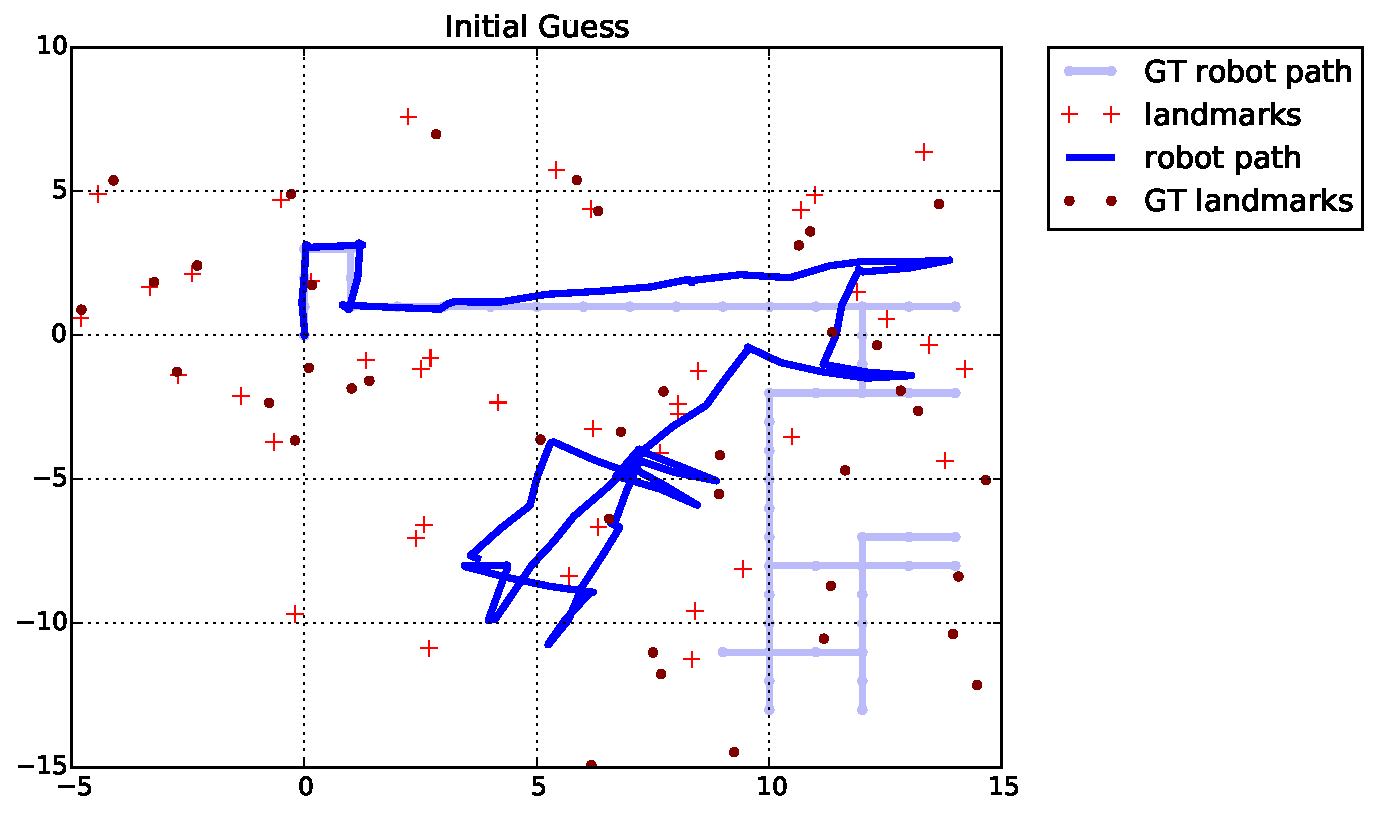
\includegraphics[width=0.8\textwidth]{imagenes/guess_op_100_oa_100_lp_100_ds_100.pdf}
    \caption{Example of an initialization of a SLAM simulation. The light blue line is ground truth path, and dark red circles are ground truth landmark. The blue line is odometry path, and red crosses are the initial guess for landmarks.}
    \label{fig:simulation}
\end{figure}

The pseudocode for the known correspondence case is shown in Algorithm~\ref{alg:known-correspondence}.

\begin{algorithm}[htbp!]
    \caption{GraphSLAM Known Correspondence}
    \label{alg:known-correspondence}
    \begin{algorithmic}[1]
        \Require optimizer, data
        \State optimizer.setParameters(parameters)
        \State optimizer.loadData(data)
        \State optimizer.genInitialGuess()
        \State optimizer.solve(numberIterations)
        \State optimizer.writeData()
    \end{algorithmic}
\end{algorithm}

Optionally g$^2$o can use robust kernels to deal with outliers. An outlier is a corrupt measurement that doesn't follows the distribution assumed for the model. They are usually generated by sensors malfunctions and tend to have extreme values, far away form the expected measurement. 

From equation~\eqref{eq:simplified}, it can be seen that each error function has a quadratic influence in function $F(\bs{y})$. This means that a single outlier can significantly degrade the construction of $F$, and thus the result of the estimation. To mitigate this problem a robust kernel function can be applied to each error term $\bs{e}_{ij}(\bs{y})$ in~\eqref{eq:simplified}, so that high values of $\bs{e}_{ij}$ has reduced effect in $F$. Robust kernels included in g$^2$o are: Cauchy, DCS, Fair, GemanMcClure, Huber, PseudoHuber, Saturated, Tukey, Welsch. Most robust kernels must also specify the kernel's width, that is the point on the function in which the kernel effect start. Figure~\ref{fig:kernels} shows the plots of different kernels in g$^2$o. 

\begin{figure}[htbp!]
    \centering
    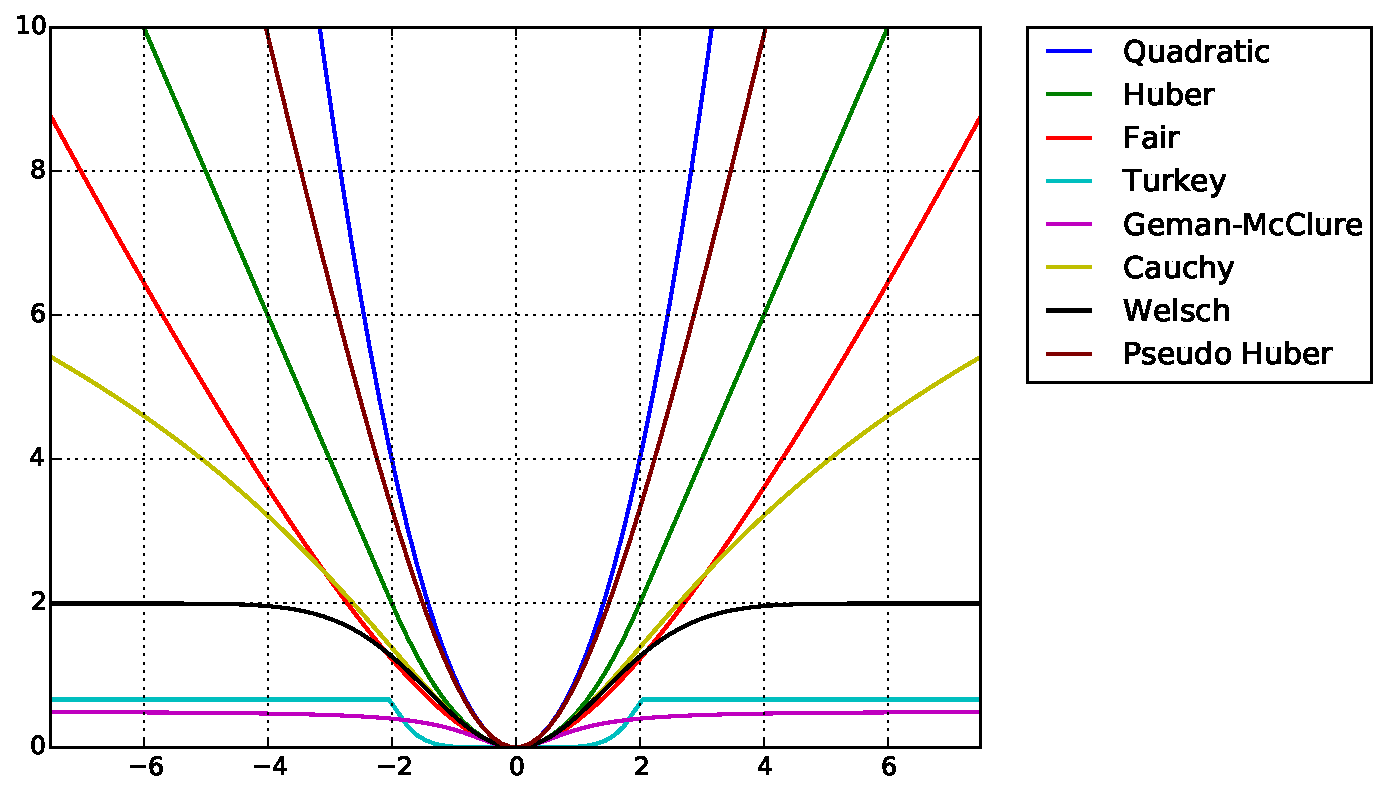
\includegraphics[width=0.8\textwidth]{imagenes/kernels.pdf}
    \caption{Plots of different robust kernels with equals width, compared with the quadratic function.}
    \label{fig:kernels}
\end{figure} 

In this work a Huber kernel of width 1 is used.

\section{The Unknown Correspondence Case}

In the unknown correspondence case there is no information of which landmark generates each measurement, neither of how many landmarks are in the map. The g$^2$o framework does not provides a way to solve the correspondence problem, so a method must be developed to address the issue. In this work the method implemented is based in the one presented in~\cite{graphslam}, with some differences to take in account the speed, and false alarms\todo{review}. 

\subsection{The Correspondence Test}

The premise of the method is as follows: a correspondence test is developed to check the likelihood of two landmarks being the same. If the likelihood is high enough, the landmarks are merged into one. 

To justify mathematically this test, the variable $\bs{\Delta}_{j,k}=\bs{m}_j-\bs{m}_k$ is defined as the difference in position of landmark $\bs{m}_j$ and $\bs{m}_k$. The posterior probability of $\bs{\Delta}_{j,k}$ over the measurements and control inputs is given by:

\begin{equation}
p(\bs{\Delta}_{j,k}|\bs{z}_{1:k},\bs{u}_{1:k})=
\det(2\pi \bs{\Sigma}_{\bs{\Delta}_{j,k}})^{-\frac{1}{2}}\exp\left\lbrace -\frac{1}{2}(\bs{\Delta}_{j,k}-\bs{\mu}_{\bs{\Delta}_{j,k}})^T
\bs{\Sigma}_{\bs{\Delta}_{j,k}}^{-1}(\bs{\Delta}_{j,k}-\bs{\mu}_{\bs{\Delta}_{j,k}})\right\rbrace
\label{eq:correspondence-test}
\end{equation}

Where $\bs{\mu}_{\bs{\Delta}_{j,k}}$ is the current estimate of the landmark's difference. It can be easily computed as $\bs{\mu}_{\bs{m}_j}-\bs{\mu}_{\bs{m}_k}$, where $\bs{\mu}_{\bs{m}_j}$ and $\bs{\mu}_{\bs{m}_k}$ are the current estimate of both landmarks.

Matrix $\bs{\Sigma}_{\bs{\Delta}_{j,k}}$ is the covariance matrix marginalized over landmarks $j$ and $k$. Since it has been assumed a normal distribution for the estimate, $\bs{\Sigma}_{\bs{\Delta}_{j,k}}$ can be computed using the marginalization lemma~\cite{graphslam}. In practice, g$^2$o provides a function to compute $\bs{\Sigma}_{\bs{\Delta}_{j,k}}$.

\todo[inline]{explain marginal cov equation?}

When two landmarks are equivalent it is expected that their position is the same, hence $\Delta_{j,k}=0$. Evaluating this in the posterior probability~\eqref{eq:correspondence-test} gives the likelihood of landmark equivalence:

\begin{equation}
\pi_{j=k} \defi
p(\bs{\Delta}_{j,k}=0|\bs{z}_{1:k},\bs{u}_{1:k})=
\det(2\pi\bs{\Sigma}_{\bs{\Delta}_{j,k}})^{-\frac{1}{2}}
\exp\left\lbrace-\frac{1}{2}\bs{\mu}_{\bs{\Delta}_{j,k}}^T\bs{\Sigma}_{\bs{\Delta}_{j,k}}^{-1}\bs{\mu}_{\bs{\Delta}_{j,k}}\right\rbrace
\label{eq:landmark-equivalence}
\end{equation}

The correspondence test consist in assert a landmark equivalence when the likelihood $\pi_{j=k}$ is greater that a user defined threshold $\chi$. Intuitively a greater threshold means being more strict in considering a landmark merging.

\subsection{The Unknown Correspondence Algorithm}

Once the correspondence test is defined, it can be used to implement an GraphSLAM algorithm with unknown data association. 

The algorithm works as follows: first all landmarks are initialized as if each measurement correspond to an individual landmark. The correspondence test is run over every possible pair of landmarks, merging landmarks that pass the test. After the tests are finished, the estimate is updated running the solver in the same way as in the case of known correspondence. After the solver, the correspondence tests are run again, and the solver is run afterward. Correspondence test and solver are alternated until no new landmark associations are found. 

Algorithm~\ref{alg:unknown-correspondence} presents the unknown correspondence algorithm in pseudocode. 

\begin{algorithm}[htbp!]
    \caption{GraphSLAM Unknown Correspondence}
    \label{alg:unknown-correspondence}
    \begin{algorithmic}[1]
        \Require optimizer, data
        \State optimizer.setParameters(parameters)
        \State optimizer.loadData(data)
        \State optimizer.genInitialGuess()
        \State
        \While{association found} 
            \ForAll{pair of landmark ($j$,$k$)} 
                \If{correspondenceTest($j$,$k$) $\geq \chi$} 
                    \State optimizer.merge($j$,$k$) 
                \EndIf 
            \EndFor
            \State optimizer.solve(numberIterations)
        \EndWhile
        \State
        \State optimizer.writeData()
    \end{algorithmic}
\end{algorithm}

\subsection{Speeding up the Unknown Correspondence Algorithm}

Algorithm~\ref{alg:unknown-correspondence} is inefficient. In particular the correspondence test is run over every pair of landmarks at each iteration. The possible pairs is quadratic in the number of landmarks, furthermore, even landmarks that are obviously not equivalent, such as landmarks greatly separated, are tested. Empirical testing have shown that the bottleneck of the algorithm is the correspondence test, in particular, the computation of the marginalized covariance $\bs{\Sigma}_{\bs{\Delta}_{j,k}}$, so is necessary call this function as less often as possible. The optimization of the algorithm is essential to run GraphSLAM in large datasets. The next subsections presents the strategies adopted to improve the algorithm performance.

\subsubsection{Incremental Optimization}

Incremental optimization is based in the following principle: landmarks measured late in the robot's path are subject to the accumulated uncertainty of all past robot's poses. This fact is can be visualized in the simulation in Figure~\ref{fig:simulation}. This has as consequence that equivalent landmarks found late in the trajectory will be merged only when all the previous estimates of the pose has already been corrected by the algorithm. Testing correspondence between these landmarks earlier is pointless, simply because their uncertainty is to high to produce an association. 

A way to deal with this problem is to test association only for landmarks measured in early poses, and then test for late poses when the path is corrected. An extreme version of this is the \emph{incremental optimization} algorithm: at each iteration consider only the current pose. Test landmarks observed in current pose with landmarks from all previous poses, and then run the solver. In the next iteration do the same for the next pose, and repeat until the last pose. Intuitively, the algorithm is incrementally correcting the path with early measured landmarks, which have low uncertainty, until all path is corrected. Figure~\ref{fig:incremental} illustrate the working of the incremental optimization for a simple example.

\begin{figure}[htbp!]
    \centering
    \begin{subfigure}[htbp!]{0.25\textwidth} 
    \centering
    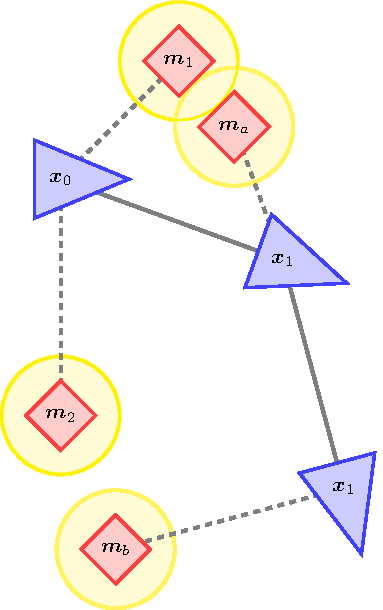
\includegraphics[width=\textwidth]{tikz/incremental1.pdf}
    \caption{Initial guess.}
    \end{subfigure}\hspace{2em}
    \begin{subfigure}[htbp!]{0.25\textwidth} 
        \centering
        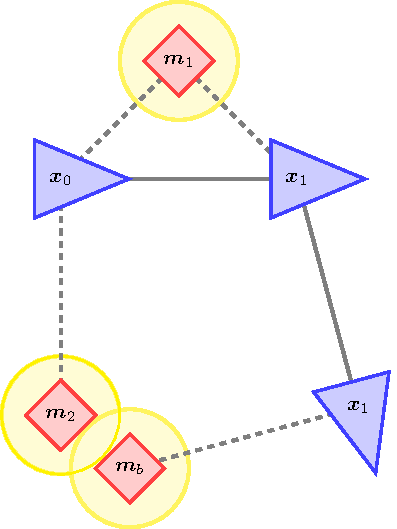
\includegraphics[width=\textwidth]{tikz/incremental2.pdf}
        \caption{Estimate after associating $m_1$ and $m_a$, and running the solver.}
    \end{subfigure}\hspace{2em}
    \begin{subfigure}[htbp!]{0.25\textwidth} 
        \centering
        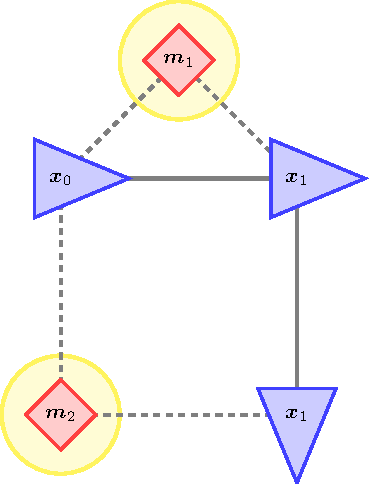
\includegraphics[width=\textwidth]{tikz/incremental3.pdf}
        \caption{Estimate after associating $m_2$ and $m_b$, and running the solver.}
    \end{subfigure}
    \caption{Example of the incremental optimization. The yellow circle represents the landmark uncertainty. Note that at first is not possible to associate landmarks $\bs{m}_2$ and $\bs{m}_b$ because $\bs{m}_b$ has the accumulated uncertainty of $\bs{x}_1$ and $\bs{x}_2$. It's not until the association between $\bs{m}_1$ and $\bs{m}_a$, observed in previous poses, is made that the latter landmarks can be merged.}
    \label{fig:incremental}
\end{figure}    
The incremental optimization has a subtle flaw, once a correspondence test is run between two landmark, it's never tested again, since only current measurements are tested. If a test failed at some point, but posterior correction make it possible for the test to pass, this association will be miss. It is expected that this situation doesn't occur often, since the incremental optimization algorithm usually gives a good estimate of the path up to the current pose. Nevertheless, this error is absolutely possible.

To mitigate this problem, \emph{full optimizations} can be run occasionally along with the incremental optimization. Full optimization consists in testing correspondence between all possible pair of measured landmarks up to the current pose, in a similar fashion as it is done in Algorithm~\ref{alg:unknown-correspondence}. This way a compromise can be achieved between the algorithm speed and performance. In this implementation the user has the is able to choose the frequency with which the full optimization are run. It is done by setting the number of incremental optimization performed between two full optimizations.  

\subsubsection{Distant Test}

Even with incremental optimization, there are still a lot of landmarks that are unnecessarily tested. The distant test strategy attempts to avoid testing landmarks that are widely separated, and thus are obviously are not equivalent. To do this, a distance threshold is defined, with which, every pair of landmarks separated by a greater distance automatically fail the test. 

Defining a value for the threshold is non trivial. Two method are implemented. The first one is by user defined input. If the user has prior knowledge of the robot or the map, he/she could make a good estimate of the maximum distance between measurements from the same landmark. Then the user can set the distance threshold to this value.

Even if the maximum distance is not known a priori, a threshold value can still be calculated. Consider the threshold $\chi$ for the correspondence test in Algorithm~\ref{alg:unknown-correspondence}, for a given value of $\chi$, there exist a distance for which, even in the best case scenario, landmarks separated by this distance or more with never be associated. To prove this, consider the random variable for the distance  $\bs{\delta}_{j,k}$ between two landmarks. Its pdf is given by:

\begin{align}
p(\bs{\delta}_{j,k}|\bs{z}_{1:k},\bs{u}_{1:k})&=
\frac{1}{\sqrt{2\pi\sigma_{\bs{\delta}_{j,k}}^2}}
\exp\left\lbrace -\frac{(\bs{\delta}_{j,k}-\bs{\mu}_{\bs{\delta}_{j,k}})^2}{2\sigma_{\bs{\delta}_{j,k}}^2}\right\rbrace\\
d_{j=k} \defi p(\bs{\delta}_{j,k}=0|\bs{z}_{1:k},\bs{u}_{1:k})&=
\frac{1}{\sqrt{2\pi\sigma_{\bs{\delta}_{j,k}}^2}}
\exp\left\lbrace -\frac{\bs{\mu}_{\bs{\delta}_{j,k}}^2}{2\sigma_{\bs{\delta}_{j,k}}^2}\right\rbrace 
\end{align}

Which is equivalent to the pdf $p(\bs{\Delta}_{j,k}|\bs{z}_{1:k},\bs{u}_{1:k})$ in \eqref{eq:correspondence-test}, for the one dimensional case. $\bs{\mu}_{\bs{\delta}_{j,k}}^2$ is the euclidean distance between the mean of the landmarks, and $\sigma_{\bs{\delta}_{j,k}}^2$ is the variance of $p(\bs{\Delta}_{j,k}|\bs{z}_{1:k},\bs{u}_{1:k})$ projected in the line between $\bs{\mu}_{\bs{\Delta}_{j,k}}^2$ and $(0,0)$. For this analysis, the exact value of $\sigma_{\bs{\delta}_{j,k}}^2$ is not important.

The maximum distance at which association can still be made is given by the following problem:

\begin{equation}
\underset{d_{j=k}\geq\chi}{\text{max}}~~  |\bs{\mu}_{\bs{\delta}_{j,k}}|
\label{eq:max-distance}
\end{equation}

Considering only the positive values of $\bs{\mu}_{\bs{\delta}_{j,k}}$, $d_{j=k}$ becomes a decreasing function. By this fact, it can be seen that maximum at~\eqref{eq:max-distance} is achieved when $d_{j=k}=\chi$. A visual demonstration of this is shown in Figure~\ref{fig:max-distance}. Expanding the equality found:

\begin{align}
d_{j=k} &= \chi\\
\frac{1}{\sqrt{2\pi\sigma_{\bs{\delta}_{j,k}}^2}}
\exp\left\lbrace -\frac{\bs{\mu}_{\bs{\delta}_{j,k}}^2}{2\sigma_{\bs{\delta}_{j,k}}^2}\right\rbrace &= \chi \\
\exp\left\lbrace -\frac{\bs{\mu}_{\bs{\delta}_{j,k}}^2}{2\sigma_{\bs{\delta}_{j,k}}^2}\right\rbrace&= \sqrt{2\pi\sigma_{\bs{\delta}_{j,k}}^2} \chi\\
\bs{\mu}_{\bs{\delta}_{j,k}} &= \sqrt{-2\sigma_{\bs{\delta}_{j,k}}^2\log(\sqrt{2\pi\sigma_{\bs{\delta}_{j,k}}^2} \chi)} \label{eq:max-distance-exp}
\end{align}

So the maximum distance for an association is given by~\eqref{eq:max-distance-exp}. Unfortunately the distance is a function of $\sigma_{\bs{\delta}_{j,k}}^2$, which is computationally expensive to get. However expression~\eqref{eq:max-distance-exp} is concave in $\sigma_{\bs{\delta}_{j,k}}^2$, so a global maximum can be found (see Figure~\ref{fig:max-variance}). Intuitively this means that neither a large nor a low value of $\sigma_{\bs{\delta}_{j,k}}^2$ is good for associating landmarks at great distances. 

\begin{figure}[htbp!]
    \centering
    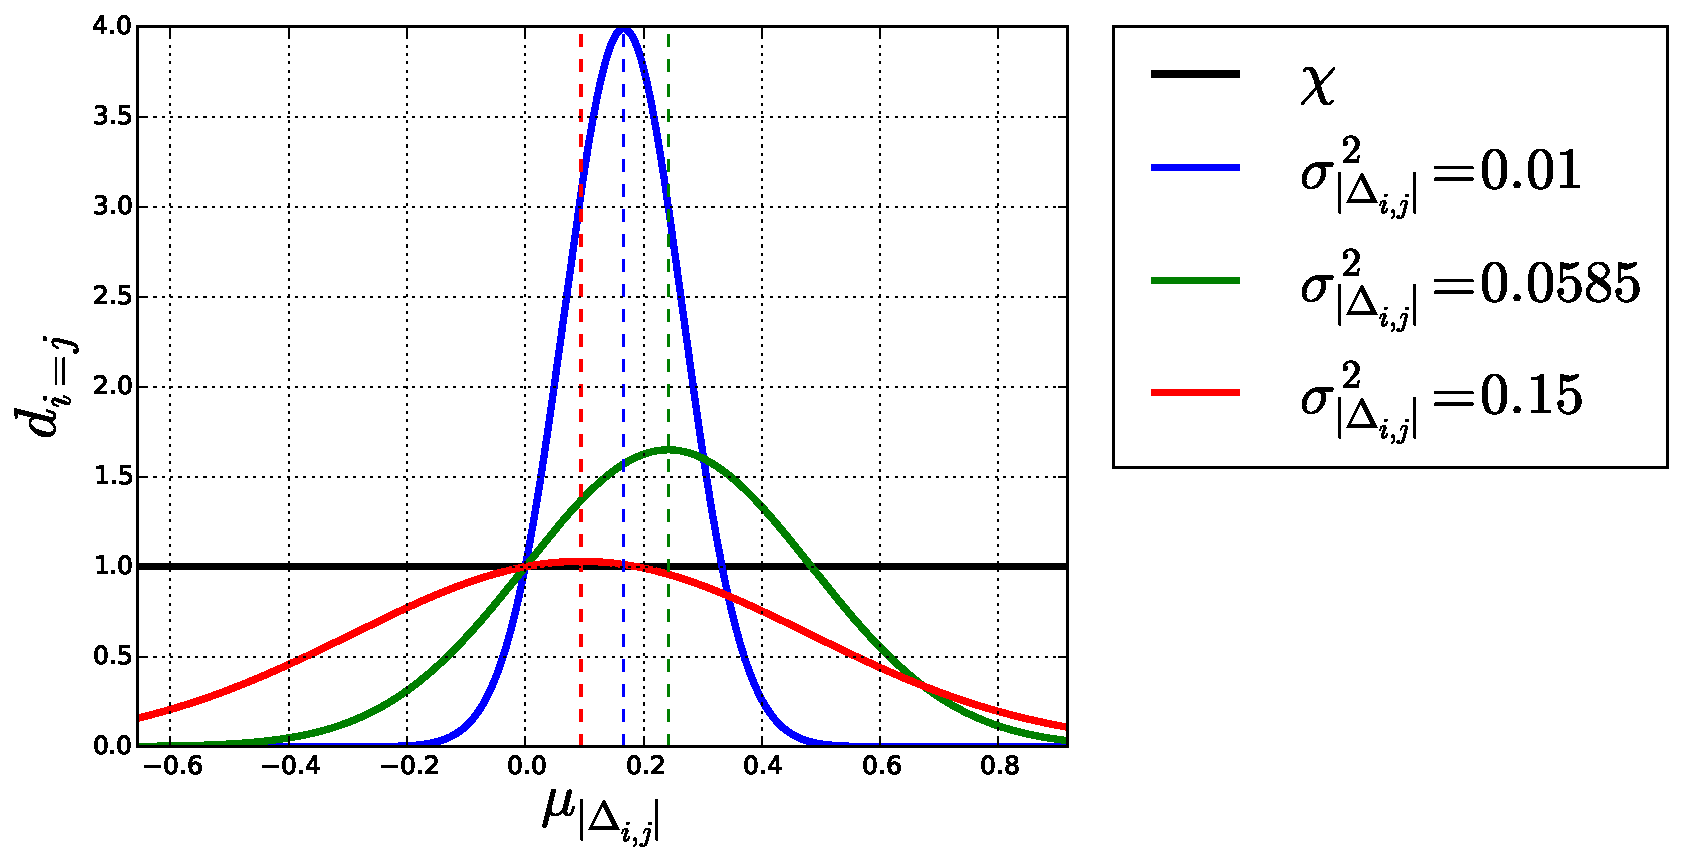
\includegraphics[width=0.7\textwidth]{imagenes/maxDistance.pdf}
    \caption{Plots of the pdf of the distance between two landmarks for different values of $\sigma_{\bs{\delta}_{j,k}}^2$. The plots shows that maximum distance from zero is achieve when, $d_{j=k}=\chi$. Note that the function that achieve more distance is neither the one with more nor with less variance.}
    \label{fig:max-distance}
\end{figure} 
\begin{figure}[htbp!]
    \centering
    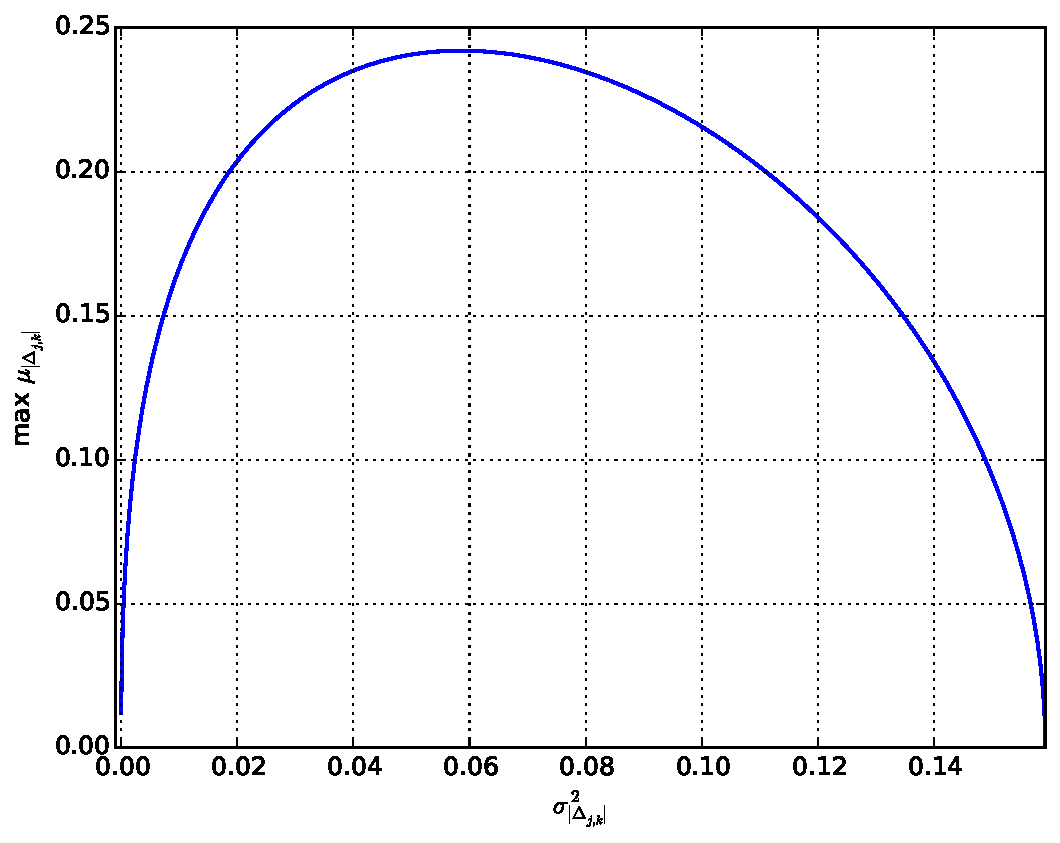
\includegraphics[width=0.5\textwidth]{imagenes/maxVariance.pdf}
    \caption{Plot of the maximum distance $\bs{\mu}_{\bs{\delta}_{j,k}}$ in function of $\sigma_{\bs{\delta}_{j,k}}^2$. It can be seen that is a concave function.}
    \label{fig:max-variance}
\end{figure} 

Using differential calculus it can be found maximum of $\bs{\mu}_{\bs{\delta}_{j,k}}$ for $\sigma_{\bs{\delta}_{j,k}}^2$ is achieved in $\sigma_{\bs{\delta}_{j,k}}^2 = \frac{1}{2\pi e\chi}$, which yields a value of $\bs{\mu}_{\bs{\delta}_{j,k}} = \frac{1}{\sqrt{2\pi e}\chi}$.  
This value can be used as a distant threshold that only depends on $\chi$. The disadvantage of this method is that the threshold computed tend to be large relative to the problem, so the amount of correspondence tests avoided is limited.

%\subsubsection{Late Landmark Merging}
